\section{The Second Wave of BCI}
\NTXDivider{The Second Wave of BCI}

\begin{frame}{Brain implants did not begin with Neuralink}
  \begin{columns}[c,onlytextwidth]
    \column{.55\textwidth}
      \small
      \NTXPoint{A longer implant history}{From cardiac pacemakers to cochlear implants and deep brain stimulation.}
      \NTXPoint{Different interfaces and purposes}{Cochlear implants stimulate the auditory nerve; DBS stimulates brain targets. Neither is synonymous with a motor BCI.}
      \NTXPoint{BCI before the headlines}{Utah arrays and BrainGate preceded Neuralink. Hochberg et al. (2006): implanted neural control of devices by a person with tetraplegia.}
    \column{.41\textwidth}
      \centering
      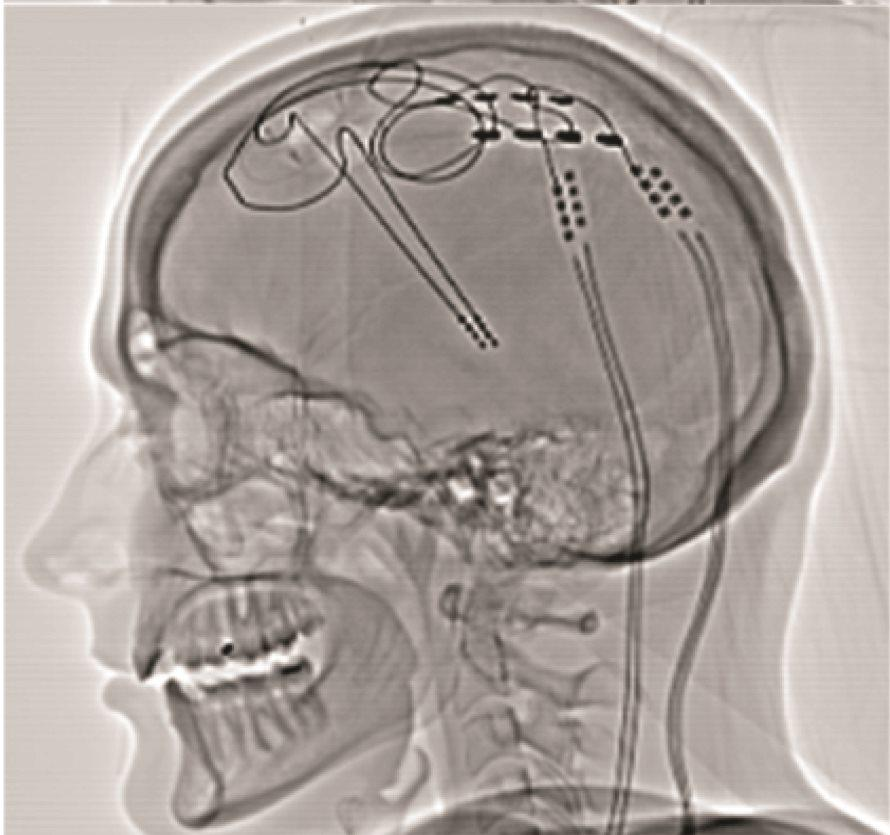
\includegraphics[width=\linewidth,height=43mm,keepaspectratio]{assets/history/india-implant-xray-000.jpg}\par\smallskip
      {\tiny Implant image reused from my NeuroTechX India talk\newline Original slide credit: Ingenia\par}
  \end{columns}
  {\tiny\color{NTXMuted}Sources: \href{https://www.nidcd.nih.gov/health/cochlear-implants}{NIDCD}; \href{https://www.ninds.nih.gov/health-information/disorders/deep-brain-stimulation-dbs}{NINDS}; \href{https://doi.org/10.1038/nature04970}{Hochberg et al., Nature, 2006}\par}
  \note{[55:15--56:45] Adapted from slides 5--18 of Morgan's NeuroTechX India presentation, Neuralink and Brain-Computer Interfaces. Begin with the implant history, not a claim that these devices are all BCIs. Cardiac pacemakers are an engineering antecedent, not brain implants. Cochlear implants act on the auditory nerve, whereas DBS electrodes deliver stimulation in brain targets. The image is carried over from slide 6, which credits Ingenia; do not identify it as a Neuralink device or infer a patient diagnosis or exact implant model. BrainGate's 2006 paper provides a concrete human intracortical BCI milestone, not the beginning of the whole field. Omit the old deck's sweeping clinical claims, device comparisons, and relative dates.}
\end{frame}

\begin{frame}{The second wave: BCI enters the public imagination}
  \begin{columns}[c,onlytextwidth]
    \column{.53\textwidth}
      \small
      \NTXPoint{My framing: a second wave}{Elon Musk and Neuralink's marketing brought BCI into a much wider public conversation.}
      \NTXPoint{Engineering and publicity are different}{Neuralink's 2019 paper described flexible threads, insertion robotics, and custom electronics. Public attention is not clinical evidence.}
      \NTXPoint{The community opportunity}{Turn that curiosity into learning, open projects, and informed founders --- while keeping expectations grounded.}
    \column{.43\textwidth}
      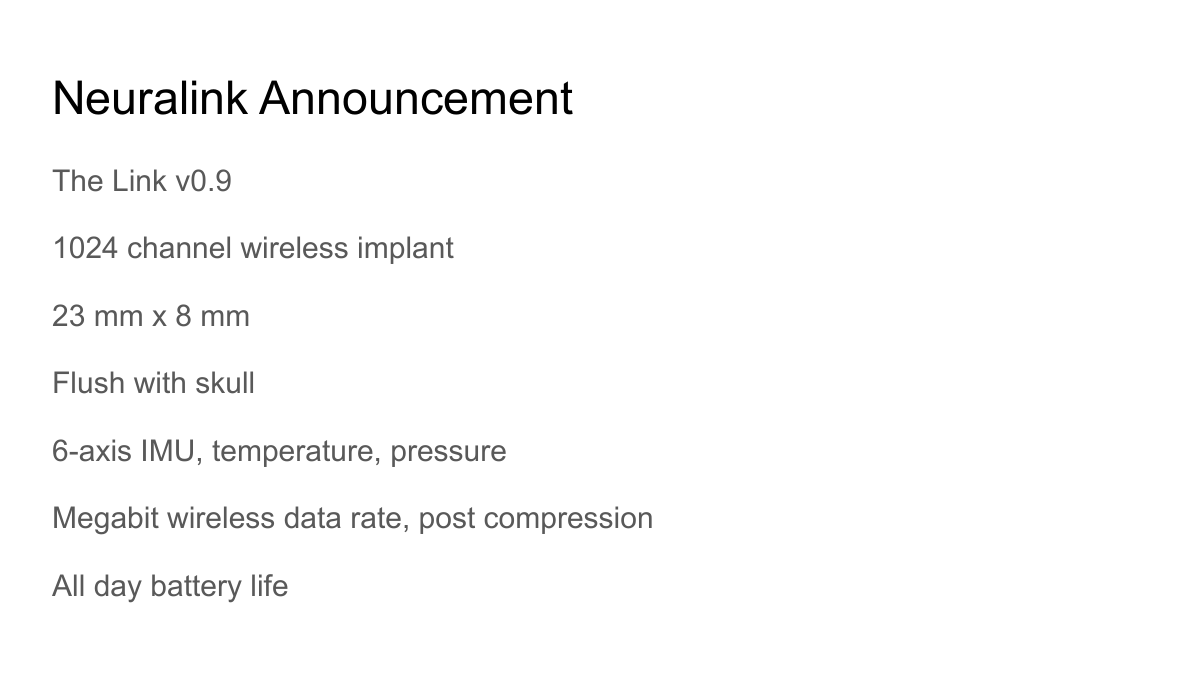
\includegraphics[width=\linewidth,height=40mm,keepaspectratio]{assets/history/india-neuralink-announcement-historical.png}\par\smallskip
      {\scriptsize From my NeuroTechX India presentation\par}
      {\tiny Historical Link v0.9 announcement slide\newline Not current specifications or verified clinical outcomes\par}
  \end{columns}
  {\tiny\color{NTXMuted}Sources: \href{https://docs.google.com/presentation/d/1tg9bppwmBDEhUSRyLswBP6Aj8QDDXgv3TXCEmOl_0yQ/edit}{Morgan Hough, NeuroTechX India deck}; \href{https://doi.org/10.2196/16194}{Musk \& Neuralink, JMIR, 2019}. ``Second wave'': Morgan's interpretation.\par}
  \note{[56:45--58:15] This is Morgan's proposed second-wave narrative, not a standard historical taxonomy or a claim that Neuralink invented BCI. The original India deck discussed Link v0.9 announcements alongside predecessors and competitors. The inset is an archival reproduction of slide 18, not an endorsement of its announcement claims as measured performance. Do not read its numbers as current product specifications. Distinguish the 2019 research platform in the cited paper from the later Link v0.9 announcement. The marketing/public-awareness argument is Morgan's interpretation; no quantitative attribution of investment or recruitment is asserted. Connect this discussion back to NeuroTechX: attention can bring people through the door, but learning, collaboration, and evidence help them become contributors and founders.}
\end{frame}

\begin{frame}{InterfaceNeuro: bringing the implant ecosystem together}
  \begin{columns}[c,onlytextwidth]
    \column{.52\textwidth}
      \small
      \NTXPoint{From InterfaceRice to InterfaceNeuro}{A joint Rice--Georgia Tech meeting series connecting research, engineering, medicine, and industry.}
      \NTXPoint{2025: Georgia Tech, May 7--8}{Brain, body, and machine interfaces; \emph{Wired Lives} brought implanted-BCI users' stories into the conversation.}
      \NTXPoint{2026: Rice, May 19--20}{Translational brain research, chronic BCI implants, and the wider social context.}
    \column{.44\textwidth}
      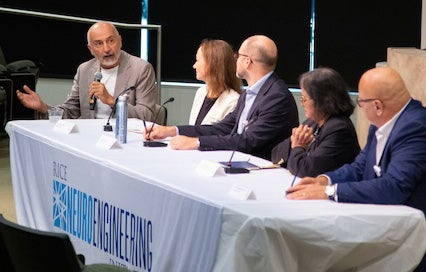
\includegraphics[width=\linewidth,height=40mm,keepaspectratio]{assets/history/interfaceneuro-rice-2026.jpg}\par\smallskip
      {\tiny InterfaceNeuro 2026, Rice University\newline Photo: Donald Soward / Rice University\par}
  \end{columns}
  {\tiny\color{NTXMuted}Sources: \href{https://inc.rice.edu/about}{Conference history}; \href{https://inc.rice.edu/}{InterfaceNeuro}; \href{https://news.rice.edu/news/2026/rice-hosts-translational-brain-research-conference}{Rice 2026 report / photo}\par}
  \note{[58:15--59:45] InterfaceNeuro and the Rice/Georgia Tech meetings are a connected series, not three independent conferences. The official history documents InterfaceRice in 2024, InterfaceNeuro at Georgia Tech on May 7--8, 2025, and the 2026 Rice event on May 19--20. The history page's odd/even-year description contradicts those dated events; use the actual dates, not that rule. The 2025 Story Collider event Wired Lives included people living with implanted BCIs. Rice's 2026 recap confirms multidisciplinary participation and credits Donald Soward for this panel photo. These meetings illustrate where sustained dialogue follows public interest in implants; no NTX ownership, partnership, or Morgan attendance is inferred.}
\end{frame}

\begin{frame}{Follow the methods communities: Lead-DBS and NEURAL}
  \begin{columns}[c,onlytextwidth]
    \column{.55\textwidth}
      \small
      \NTXPoint{Lead-DBS: recurring participation}{Developer meetings, workshops, shared code, and support around DBS imaging and analysis.}
      \NTXPoint{Bordeaux: learning the disconnectome}{NEURAL workshops with Michel Thiebaut de Schotten and colleagues; 2025 and June 8--12, 2026.}
      \NTXPoint{Stay connected beyond the headlines}{Follow the meetings, learn the tools, and contribute to the communities doing the methodological work.}
    \column{.41\textwidth}
      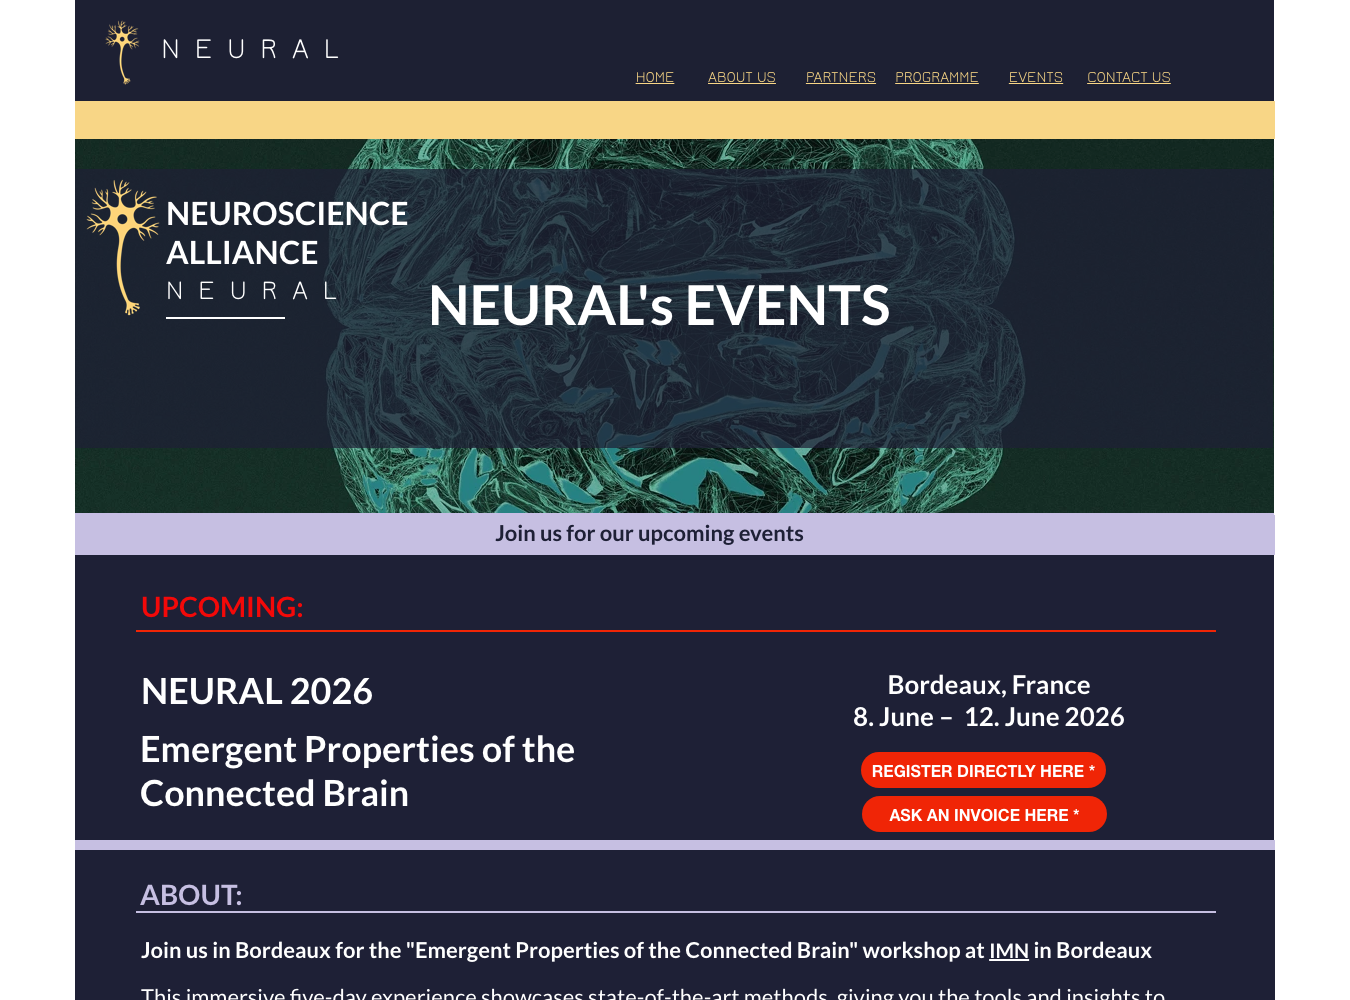
\includegraphics[width=\linewidth,height=43mm,keepaspectratio]{assets/history/neural-bordeaux-2026-page.png}\par\smallskip
      {\tiny NEURAL: Emergent Properties of the Connected Brain\newline Official page; June 2026 event is now past\par}
  \end{columns}
  {\tiny\color{NTXMuted}Sources: \href{https://netstim.gitbook.io/leaddbs/ways-to-contribute-to-lead-dbs}{Lead-DBS community}; \href{https://www.lead-dbs.org/helpsupport/workshops/}{workshops}; \href{https://storage.googleapis.com/bcblabweb/events.html}{NEURAL program}\par}
  \note{[59:45--61:15] Lead-DBS's contributor guide invites people to monthly developer meetings coordinated on Slack; its workshop archive documents hands-on training. This is an imaging and analysis community, not an implanted motor-BCI product. The French meeting is identified here as NEURAL, Emergent Properties of the Connected Brain, in Bordeaux. Stephanie Forkel's institutional record documents the October 2025 edition; the organizer page lists June 8--12, 2026, with Michel Thiebaut de Schotten teaching the disconnectome, alongside Valentina Pacella, Stephanie Forkel and Anna Matsulevits. Its stale Upcoming label should not be repeated in a September talk. Disconnectome methods concern network disconnection, including after lesions; they are not synonymous with DBS targeting or BCI decoding. These are related communities to follow, not NTX programs or proof of clinical effectiveness.}
\end{frame}
